\section{Problem Description and Mathematical Model}\label{sec:model}
\subsection{System Definition and Assumptions}
Several lines process different end-of-life products while drawing humans and robots from shared pools. Fig.~\ref{fig:product} illustrates a serviceable electric fan unit and its recovery operations. It is a conceptual example for explaining task relationships, not an industrial measurement or an experimental input. Each line has an AND precedence graph. An executed successor requires every direct predecessor. Optional tasks can remain unexecuted; required tasks must be executed.

The illustrative tasks remove the front guard ($T_1$), detach the impeller ($T_2$), open the rear cover ($T_3$), disconnect the controller ($T_4$), extract the motor unit ($T_5$), separate the rotor ($T_6$), recover the stator ($T_7$), and recover the power lead ($T_8$). These labels connect the component tree to the access graph.

\begin{figure}[!t]\centering
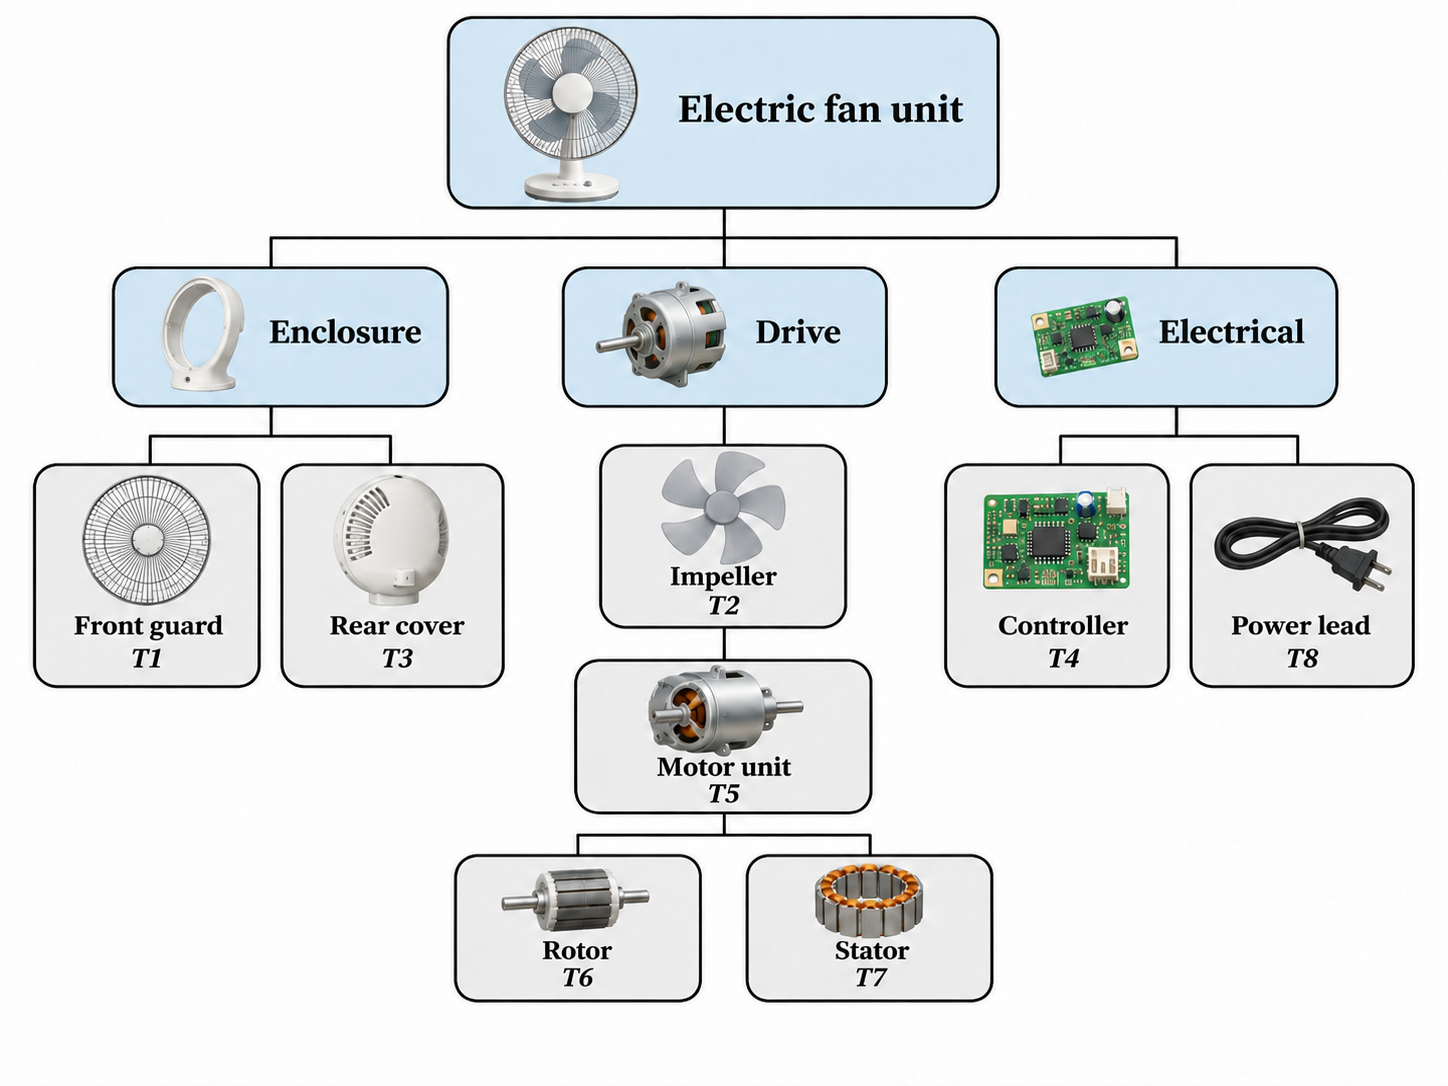
\includegraphics[width=\columnwidth]{img/product_structure.png}
\caption{Illustrative fan-unit product structure and recovery operations. The component tree indicates containment, not precedence; the task graph in Fig.~\ref{fig:andor} defines access dependencies.}\label{fig:product}
\end{figure}

Fig.~\ref{fig:ring} shows a physical circular layout. A fixed entry cuts each circle into ordered stations. A product visits these stations once and exits; only empty carriers return. Consequently, station indices have the same precedence meaning as an ordered line. The model contains no multi-lap product routing, geometric travel time, or cyclic task sequence. The figure illustrates the adopted layout without changing the underlying assignment constraints.

\begin{figure}[!t]\centering
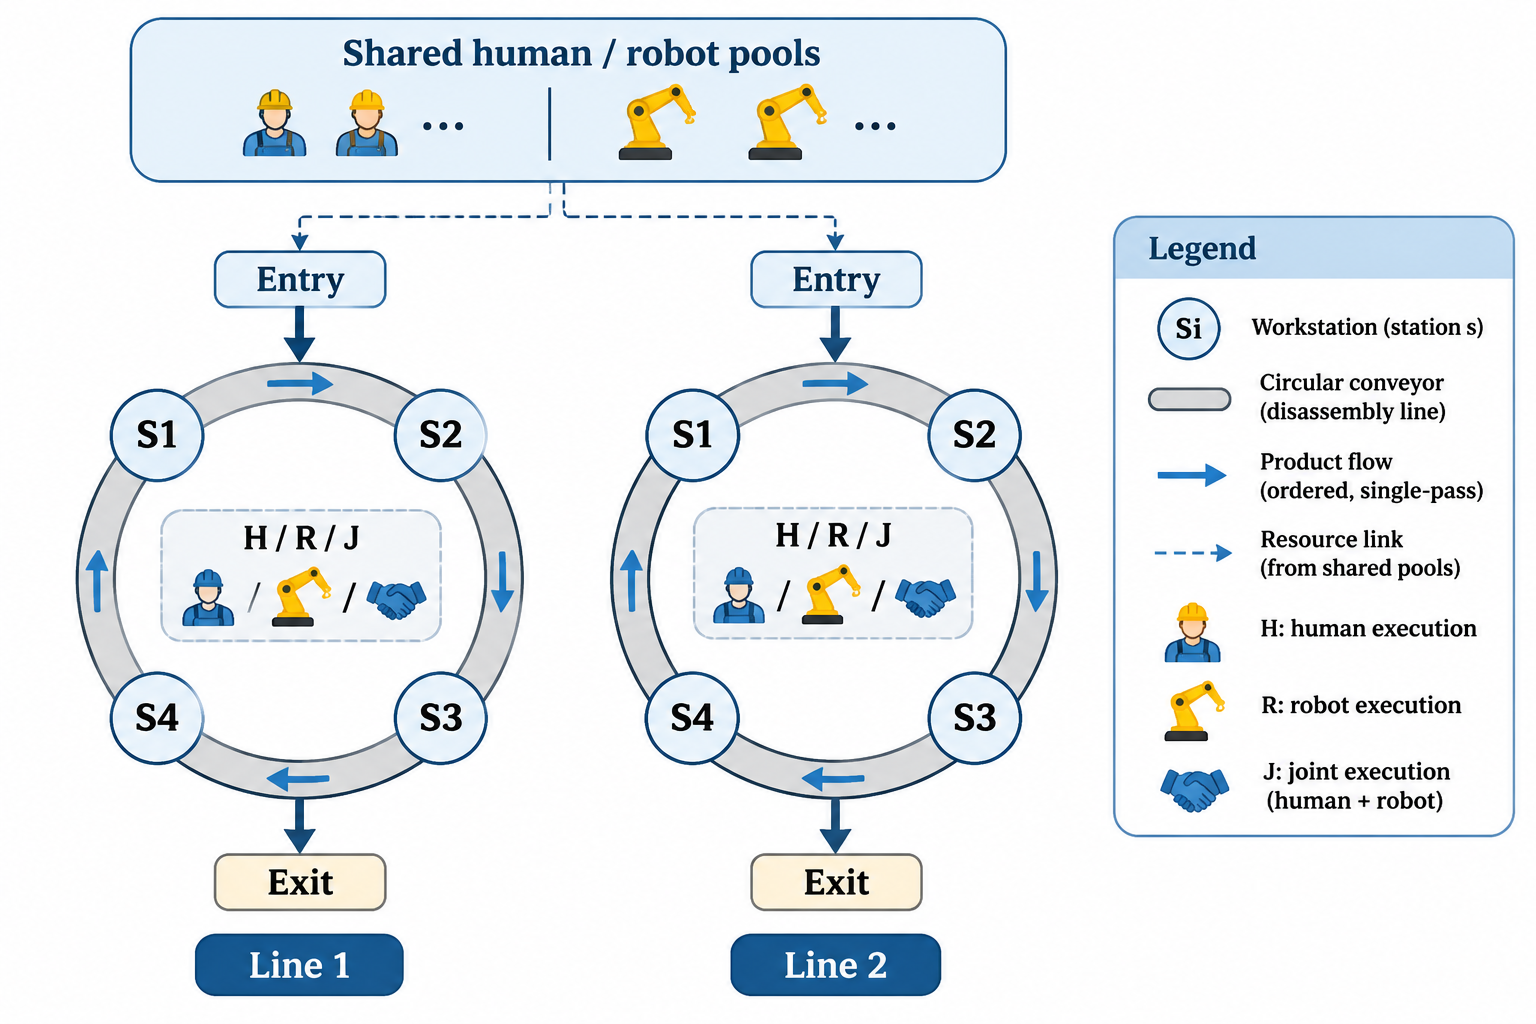
\includegraphics[width=\columnwidth]{img/circular_lines.png}
\caption{Two illustrative circular lines with fixed entry, ordered single-pass processing, and shared planning pools. Dashed return arcs carry empty carriers only. Pool links indicate deployment limits, not movement during operation.}\label{fig:ring}
\end{figure}

Modes H, R, and J denote human, robot, and joint execution. Mode J requires one human and one robot; its duration enters station time once. Tasks within a station execute sequentially. A selected task receives exactly one allowed mode at exactly one station. Fig.~\ref{fig:andor} distinguishes AND access dependencies from the OR choice among execution modes. OR does not denote mutually exclusive product-disassembly routes. A predecessor can share a station with its successor; a topological order gives a feasible within-station sequence.

\begin{figure}[!t]\centering
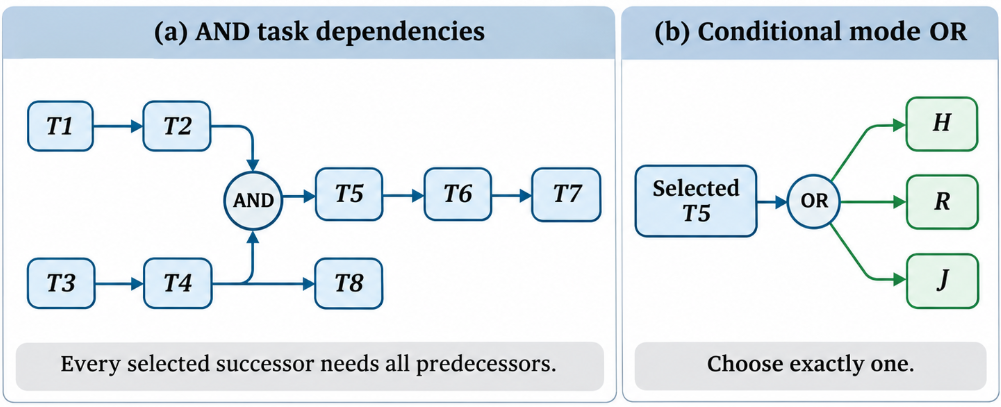
\includegraphics[width=\columnwidth]{img/and_mode_or.png}
\caption{Illustrative AND dependencies and conditional execution-mode OR. Both $T_2$ and $T_4$ precede $T_5$. If $T_5$ is selected, exactly one allowed mode is chosen; omitting an optional task selects none. The diagram introduces no route-selection OR constraint.}\label{fig:andor}
\end{figure}

Fatigue starts at zero in a representative cycle. Each human-involving task contributes a nonnegative additive load. There is no within-cycle recovery or accumulation across successive cycles. Robot-only modes have zero fatigue load. Resource pools limit the total number of stations with human and robot deployment. This planning model does not describe resource movement. Candidate stations can have different costs, and consecutive activation is not required. There are no precedence arcs between lines.

\subsection{Notation}
\subsubsection{Sets and indices}
\begin{description}[\IEEEsetlabelwidth{$\mathcal I_l^{\rm req}$:}\setlength{\labelsep}{0.6em}\raggedright]
\item[$\mathcal L$:] Set of disassembly lines, indexed by $l$.
\item[$\mathcal I_l$:] Tasks on line $l$, indexed by $i,j$; $n_l=|\mathcal I_l|$.
\item[$\mathcal I_l^{\rm req}$:] Subset of required tasks on line $l$.
\item[$\mathcal S_l$:] Ordered candidate stations $\{1,\ldots,k_l\}$, indexed by $s$; $k$ denotes a station prefix endpoint.
\item[$\mathcal M_{li}$:] Allowed modes for task $i$, a subset of $\{H,R,J\}$, indexed by $m$.
\item[$\mathcal E_l$:] Direct AND arcs $(i,j)$, where $i$ precedes $j$.
\end{description}
\subsubsection{Parameters}
\begin{description}[\IEEEsetlabelwidth{$c_{ls}^{0},c_{ls}^{H},c_{ls}^{R}$:}\setlength{\labelsep}{0.6em}\raggedright]
\item[$v_{li},w_{li}$:] Recovery value and recovery weight of task $i$.
\item[$c_{li}^{m},t_{li}^{m}$:] Direct execution cost and processing duration in mode $m$.
\item[$\beta_{li}^{m}$:] Fatigue coefficient; $d_{li}^{m}=\beta_{li}^{m}t_{li}^{m}$ is the corresponding load.
\item[$c_{ls}^{0},c_{ls}^{H},c_{ls}^{R}$:] Station activation, human deployment, and robot deployment costs.
\item[$t_l^c$:] Cycle-time limit on line $l$.
\item[$\bar f_l,b_l$:] Fatigue threshold and additive budget, with $0\leq\bar f_l<1$ and $b_l=-\ln(1-\bar f_l)$.
\item[$q_l$:] Minimum recovered weight on line $l$.
\item[$h^{\max},r^{\max}$:] Shared human and robot capacities.
\item[$a_m^H,a_m^R$:] Resource indicators, equal to $(1,0)$ for H, $(0,1)$ for R, and $(1,1)$ for J.
\end{description}
\subsubsection{Decision variables}
\begin{description}[\IEEEsetlabelwidth{$h_{ls},r_{ls}$:}\setlength{\labelsep}{0.6em}\raggedright]
\item[$y_{li}$:] One if task $i$ is selected, and zero otherwise.
\item[$x_{lism}$:] One if task $i$ executes at station $s$ in mode $m$.
\item[$u_{ls}$:] One if station $s$ is active.
\item[$h_{ls},r_{ls}$:] Human and robot deployment indicators at station $s$.
\end{description}

\subsection{Compact Formulation}
Every sum over $m$ uses the task's allowed set $\mathcal M_{li}$. Unless a row states otherwise, task rows apply to all $l,i$ and station rows to all $l,s$. Net profit is maximized:
\begin{align}
\max\ z={}&\sum_{l,i}v_{li}y_{li}-\sum_{l,i,s,m}c_{li}^{m}x_{lism}\nonumber\\
&-\sum_{l,s}\left(c_{ls}^{0}u_{ls}+c_{ls}^{H}h_{ls}+c_{ls}^{R}r_{ls}\right).\label{eq:obj}
\end{align}
\begin{align}
\sum_{s\in\mathcal S_l}\sum_{m\in\mathcal M_{li}}x_{lism}&=y_{li}&&\forall l,i,\label{eq:assign}\\
y_{li}&=1&&\forall l,\ i\in\mathcal I_l^{\rm req}.\label{eq:required}
\end{align}

For every $l$, $(i,j)\in\mathcal E_l$, and $k\in\mathcal S_l$, AND precedence requires
\begin{equation}
\sum_{s=1}^{k}\sum_{m\in\mathcal M_{lj}}x_{ljsm}
\leq\sum_{s=1}^{k}\sum_{m\in\mathcal M_{li}}x_{lism}.\label{eq:prec}
\end{equation}
\begin{align}
\sum_{i,m}t_{li}^{m}x_{lism}&\leq t_l^c u_{ls},\label{eq:cycle}\\
u_{ls}\leq\sum_{i,m}x_{lism}&\leq n_lu_{ls},\label{eq:active}\\
h_{ls}\leq\sum_{i,m}a_m^Hx_{lism}&\leq n_lh_{ls},\label{eq:hlogic}\\
r_{ls}\leq\sum_{i,m}a_m^Rx_{lism}&\leq n_lr_{ls},\label{eq:rlogic}\\
\sum_{i,m}d_{li}^{m}x_{lism}&\leq b_lh_{ls}.\label{eq:fatigue}
\end{align}

\begin{align}
\sum_{l,s}h_{ls}&\leq h^{\max},\label{eq:sharedh}\\
\sum_{l,s}r_{ls}&\leq r^{\max},\label{eq:sharedr}\\
\sum_{i\in\mathcal I_l}w_{li}y_{li}&\geq q_l&&\forall l,\label{eq:recovery}\\
x_{lism},y_{li},u_{ls},h_{ls},r_{ls}&\in\{0,1\}.\label{eq:binary}
\end{align}

Objective~\eqref{eq:obj} subtracts execution, station, human, and robot costs from task recovery value.

Constraint~\eqref{eq:assign} indicates that a selected task receives exactly one station--mode assignment; an omitted task receives none. It enforces the conditional mode OR in Fig.~\ref{fig:andor}.

Constraint~\eqref{eq:required} indicates that every required task is selected.

Constraint~\eqref{eq:prec} indicates that each successor requires its predecessor at the same or an earlier station. The final prefix enforces predecessor selection. Applying the row to every incoming arc gives AND precedence.

Constraint~\eqref{eq:cycle} indicates that total station processing time does not exceed the line cycle limit when the station is active.

Constraint~\eqref{eq:active} indicates that a station is active if and only if it contains at least one task. Thus an empty station incurs no activation cost.

Constraint~\eqref{eq:hlogic} indicates that a human is deployed if and only if at least one assigned mode requires a human.

Constraint~\eqref{eq:rlogic} indicates the corresponding if-and-only-if requirement for robot deployment. Together these rows charge both resources for mode J and for a station mixing H and R tasks.

Constraint~\eqref{eq:fatigue} indicates that cumulative human load stays within its additive budget. Equivalently, the station fatigue level $1-\exp(-\sum_{i,m}d_{li}^{m}x_{lism})$ does not exceed $\bar f_l$ at a human-equipped station.

Constraint~\eqref{eq:sharedh} indicates that total human deployment across all lines does not exceed the shared capacity.

Constraint~\eqref{eq:sharedr} indicates the analogous limit for robots.

Constraint~\eqref{eq:recovery} indicates that every line meets its minimum recovered weight.

Constraint~\eqref{eq:binary} indicates the binary domains of task, assignment, activation, and deployment decisions. These definitions retain the mathematical feasible set of the implemented compact model.
